% !TeX root = ../tfg.tex
% !TeX encoding = utf8

\chapter{Símplices y complejos simpliciales}

Los espacios topológicos pueden llegar a ser complicados de estudiar. Los
complejos simpliciales tienen la ventaja de ser estructuras fáciles de estudiar.
Por este motivo, los dotaremos de cierta topología que nos permitirá construir
homeomorfismos a un gran número de espacios topológicos. En este capítulo nos centraremos
en la definición y el estudio de estos objetos en profundidad en la línea de \cite{munkres2018elements}
y lo complementaremos con alguna aportación de \cite{lee2010introduction}.

\section{Símplices}
Con la finalidad de generalizar estructuras como el triángulo y el tetraedro, a
finales del siglo XIX nace un nuevo concepto: el símplice. Su sencillez y
propiedades lo convirtieron en una herramienta muy versátil en el estudio de la
topología algebraica, dando lugar a lo que hoy conocemos como homología simplicial.
En esta sección definiremos lo que es un símplice y algunos conceptos asociados
a él que nos serán de gran utilidad en el estudio de dicho campo. Comenzamos recordando
algunos conceptos de la geometría afín.

Como tan sólo será necesario trabajar en el espacio afín usual $N$-dimensional,
lo notaremos simplemente por $\mathbb{R}^{N}$.

\begin{definicion}
	Sea $\{a_{0}, \dots, a_{p}\}$ un conjunto de puntos en $\mathbb{R}^{N}$.
	Diremos que dicho conjunto es \textbf{afínmente independiente} si para cualesquiera
	$t_{i} \in \mathbb{R}$, las ecuaciones
	\[
	\sum_{i=0}^{p}t_{i}=0 \quad \text{y}\quad \sum_{i=0}^{p}t_{i}a_{i}=0
	\]
	implican que $t_{0} = t_{1} = \dots = t_{p}$.
\end{definicion}

\begin{definicion}
	Sea $\{a_{0}, \dots, a_{p}\}$ un conjunto de puntos afínmente independiente.
	Definimos el \textbf{plano afín} $P$ generado por $\{a_{0}, \dots, a_{p}\}$ como
	el conjunto de puntos $x \in \mathbb{R}^{N}$ tales que
	\[
	x = \sum_{i=0}^{p}t_{i}a_{i} = a_{0} + \sum_{i=1}^{p}t_{i}(a_{i} - a_{0})
	\]
	para algunos $t_{1}, \dots, t_{p} \in \mathbb{R}$. Diremos entonces que $P$ es
	el plano que pasa por $a_{0}$ paralelo a los vectores $a_{i} - a_{0}$, $i \in \{
	1, \dots, p\}$.
\end{definicion}

Nótese que la transformación afín $T$ de $\mathbb{R}^{N}$ tal que
$T(x) = x - a_{0}$ es una traslación que lleva el plano $P$ al subespacio
vectorial de $\mathbb{R}^{N}$ con base
$a_{1}-a_{0}, a_{2}-a_{0}, \dots, a_{p}-a_{0}$. Si componemos dicha transformación
con una aplicación lineal que lleve cada vector $a_{1}-a_{0}, a_{2}-a_{0}, \dots,
a_{p}-a_{0}$ a los primeros $N$ vectores de la base usual, obtenemos una
transformación afín $S: P \rightarrow \R^{N} \times \{0\}$ tal que
$S(a_{i}) = (0, \overset{i-1}{\dots}, 0, 1, 0, \overset{i+1}{\dots}, 0)$ con
$i \in \{1, \dots, p\}$.

\begin{definicion}
	\label{def:simplex}
	Sea $\{a_{0}, \dots, a_{p}\}$ un conjunto de puntos afínmente independiente en
	$\mathbb{R}^{N}$. Definimos el \textbf{p-símplice} o \textbf{símplice}
	$\sigma = [a_{0}, \dots, a_{p}]$ generado por $a_{0}, \dots, a_{p}$ como el
	conjunto de todos los $x \in \mathbb{R}^{N}$ tales que
	\[
	x=\sum_{i=0}^{p}t_{i}a_{i} \quad \text{y}\quad \sum_{i=0}^{p}t_{i}=1
	\]
	con $t_{i} \geq 0$, $i \in \{0, 1, \dots, p\}$. Diremos que $t_i$ es la \textbf{$i$-ésima coordenada baricéntrica} de $x$ respecto a $a_0, a_1, \ldots, a_p$.
\end{definicion}

\begin{proposicion}
	Sea $\sigma$ un $k$-símplice definido como en \ref{def:simplex}.
	Entonces, para cualquier $p \in \sigma$, las coordenadas baricéntricas
	$t_{0}, \ldots, t_{k}$ de $p$ están determinadas de manera única.
\end{proposicion}
\begin{proof}
	Por definición, cualquier punto arbitrario $p \in \sigma$ puede escribirse
	como una combinación convexa de los puntos $a_{i}$. Esto garantiza la existencia
	de una solución (no negativa) al sistema lineal
	\[
	At= \left(
	\begin{array}{ccc}
		a_{01} & \cdots & a_{k1} \\
		\vdots & \ddots & \vdots \\
		a_{0N} & \cdots & a_{kN} \\
		1      & \cdots & 1
	\end{array}
	\right) \left(
	\begin{array}{c}
		t_0    \\
		\vdots \\
		t_k
	\end{array}
	\right) = \left(
	\begin{array}{c}
		p_1    \\
		\vdots \\
		p_N    \\
		1
	\end{array}
	\right) = p^{*},
	\]
	donde $A$ es la matriz que contiene a los $a_{i}$ como columnas, extendidos
	con un $1$ en la última fila para incorporar la condición de que la suma de
	$t_{i}$ sea igual a $1$, asegurando que estamos considerando combinaciones convexas.
	
	Para demostrar la unicidad, supongamos la existencia de otro vector
	$t'$ tal que $A t'= p^{*}$. Esto lleva a $A(t - t'
	) = 0$. Supongamos que $A(t - t') = A v = 0$, donde $v
	= t - t'$. Esto implica que para $v_{i} = t_{i} - t_{i}'$
	para todo $i \in \{0, \dots, k\}$
	\[
	\sum_{i=0}^{k}v_{i} \cdot \left(
	\begin{array}{c}
		a_{0i} \\
		\vdots \\
		a_{ki} \\
		1
	\end{array}
	\right) = 0,
	\]
	lo que lleva a que $v_{0} = v_{1} = \cdots = v_{k} = 0$, debido a la independencia
	lineal de las columnas de $A$. En consecuencia, $t= t'$,
	demostrando así que las coordenadas baricéntricas son únicas para cualquier
	punto $p$ en $\sigma$.
\end{proof}

Los puntos $a_{0}, \dots, a_{p}$ que generan $\sigma$ los llamaremos \textbf{vértices}
de $\sigma$ y al número $p$ lo llamaremos la \textbf{dimensión} de $\sigma$, que
notaremos por $\dim \sigma$.

\begin{definicion}
	Sea $\sigma=[a_{0}, \dots, a_{p}]$ un símplice. Una \textbf{cara de dimensión
		$p$} de $\sigma$ será cualquier símplice generado por un subconjunto no vacío de
	$\{a_{0}, \dots, a_{p}\}$.
\end{definicion}
En particular, la cara de $\sigma$ generada por
$a_{0}, \dots, a_{i-1}, a_{i+1}, \dots, a_{p}$ la llamamos la \textbf{cara
	opuesta} de $a_{i}$, $i \in \{0, \dots, p\}$. Las caras de $\sigma$ diferentes de
$\sigma$ diremos que son \textbf{caras propias} de $\sigma$ y la unión de todas
ellas la llamaremos el \textbf{borde} de $\sigma$ y lo notaremos $\text{Bd}\ \sigma$.
Finalmente, definimos el \textbf{interior} de $\sigma$, $\text{Int}\ \sigma$,
como el conjunto de puntos de $\sigma$ que no pertenecen a su borde.

En ocasiones, para dos símplices $\sigma$ y $\tau$, escribiremos $\tau \preceq \sigma$ si $\tau$ es cara de $\sigma$. En caso de ser cara propia, lo notaremos por $\tau \prec \sigma$.

\begin{figure}[h]
	\begin{subfigure}
		{.24\textwidth}
		\centering
		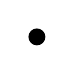
\begin{tikzpicture}
			% 3-símplice
			\node (n0) at (0.0, 0.0) {}; % root
			
			% DRAW NODES
			\draw[color=black, fill=black] (n0) circle (.1);
		\end{tikzpicture}
		\caption{0-símplice}
	\end{subfigure}
	\hfill
	\begin{subfigure}
		{.24\textwidth}
		\centering
		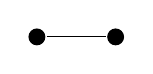
\begin{tikzpicture}
			% 3-símplice
			\node (n0) at (0.0, 0.0) {}; % root
			\node (n1) at (1.0, 0.0) {}; % extreme
			
			% DRAW TREE
			\path[draw] (n0)--(n1);
			
			% DRAW NODES
			\draw[color=black, fill=black] (n0) circle (.1); \draw[color=black, fill=black]
			(n1) circle (.1);
		\end{tikzpicture}
		\caption{1-símplice}
	\end{subfigure}
	\hfill
	\begin{subfigure}
		{.24\textwidth}
		\centering
		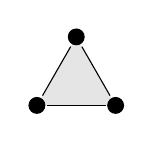
\begin{tikzpicture}
			% 3-símplice
			\node (n0) at (0.0, 0.0) {}; % root
			\node (n1) at (1.0, 0.0) {}; % extreme
			\node (n2) at (0.5, 0.87) {}; % extreme
			
			% DRAW TREE
			\fill[fill=gray!20] (n0.center)--(n1.center)--(n2.center); \path[draw] (n0)--(n1);
			\path[draw] (n1)--(n2); \path[draw] (n2)--(n0);
			
			% DRAW NODES
			\draw[color=black, fill=black] (n0) circle (.1); \draw[color=black, fill=black]
			(n1) circle (.1); \draw[color=black, fill=black] (n2) circle (.1);
		\end{tikzpicture}
		\subcaption{2-símplice}
	\end{subfigure}
	\hfill
	\begin{subfigure}
		{.24\textwidth}
		\centering
		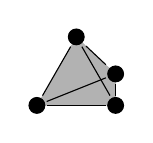
\begin{tikzpicture}
			% 3-símplice
			\node (n0) at (0.0, 0.0) {}; % root
			\node (n1) at (1.0, 0.0) {}; % extreme
			\node (n2) at (0.5, 0.87) {}; % extreme
			\node (n3) at (1.0, 0.4) {}; % inside
			
			% DRAW TREE
			\fill[fill=gray!60] (n0.center)--(n1.center)--(n2.center); \fill[fill=gray!60]
			(n0.center)--(n2.center)--(n3.center); \fill[fill=gray!60] (n0.center)--(n1.center)--(n3.center);
			\fill[fill=gray!60] (n3.center)--(n1.center)--(n2.center); \path[draw] (n0)--(n1);
			\path[draw] (n1)--(n2); \path[draw] (n2)--(n0); \path[draw] (n0)--(n3);
			\path[draw] (n1)--(n3); \path[draw] (n2)--(n3);
			
			% DRAW NODES
			\draw[color=black, fill=black] (n0) circle (.1); \draw[color=black, fill=black]
			(n1) circle (.1); \draw[color=black, fill=black] (n2) circle (.1); \draw[color=black,
			fill=black] (n3) circle (.1);
		\end{tikzpicture}
		\caption{3-símplice}
	\end{subfigure}
	\caption{Símplices de dimensión $0$, $1$, $2$ y $3$}
	\label{fig:simplex}
\end{figure}
\begin{proposicion}
	\label{prop:union-disjunta-simplices} Si $\sigma$ es un símplice, entonces es
	unión disjunta del interior de todas sus caras.
\end{proposicion}
\begin{proof}
	Sea $x$ un elemento del símplice $\sigma = [a_{0},\dots,a_{p}]$ y sean $t_{0},\dots
	,t_{p}$ sus coordenadas baricéntricas. Consideremos ahora $\sigma_{k}$ el
	símplice resultante de eliminar los vértices cuya coordenada tenía valor nulo.
	Esto es, tomamos el símplice $\sigma_{k} = [a_{i_1}, \dots, a_{i_k}]$ donde
	$t_{i_s}> 0$ para todo $s \in \{1, \dots, k\}$. Por la construcción de $\sigma_{k}$,
	tenemos que $x$ pertenece a su interior.
	
	Ahora sabemos que todo punto de un símplice pertenece al interior de una cara.
	Finalmente, la unicidad de las coordenadas baricéntricas nos garantiza que la
	unión del interior de dos caras es disjunta.
\end{proof}

Dado un símplice $\sigma$ podemos definir un orden sobre sus vértices. Dos
órdenes de $\sigma$ los consideraremos equivalentes si podemos pasar de uno a
otro con un número par de permutaciones. Así, los ordenamientos posibles para
los vértices de $\sigma$ se pueden agrupar en dos clases de equivalencia
distintas, que definimos como las \textbf{orientaciones del símplice} $\sigma$.

\begin{definicion}
	Decimos que un símplice $\sigma = [a_{0}, a_{1}, \ldots, a_{p}]$ está \textbf{orientado}
	si se le ha asignado una de estas orientaciones. Utilizaremos $[a_{0} a_{1} \ldots
	a_{p}]$ para denotar la clase de equivalencia dada por la orientación $a_{0} <
	a_{1} < \cdots < a_{p}$ del símplice generado por los vértices $a_{0},a_{1},\ldots
	, a_{p}$.
\end{definicion}

\section{Complejos simpliciales}

La importancia de los complejos simpliciales reside en su capacidad para
descomponer espacios topológicos en componentes manejables, permitiendo un análisis
detallado de su estructura. Al considerar la forma en que estos símplices se
conectan y orientan entre sí, los complejos simpliciales facilitarán la definición
de cadenas y ciclos simpliciales que serán indispensables en el estudio de la homología
simplicial.

\begin{definicion}
	Un \textbf{complejo simplicial} (finito) $K$ en $\mathbb{R}^{N}$ es una
	colección finita de símplices en $\mathbb{R}^{N}$ tal que:
	\begin{enumerate}
		\item Toda cara de un símplice de $K$ está en $K$.
		
		\item La intersección de cualesquiera dos símplices de $K$ o es el vacío o es
		una cara de ambos símplices.
	\end{enumerate}
\end{definicion}
\begin{nota}
	Si bien los complejos simpliciales se pueden formular sin la restricción de finitud,
	nosotros trabajaremos solamente en el caso finito por conveniencia en algunos
	resultados.
\end{nota}

En ciertas ocasiones puede ser interesante saber si dada una colección
cualquiera de símplices, esta es un complejo simplicial o no. Para ello, el siguiente
lema nos puede ser de utilidad.

\begin{lema}
	Una colección $K$ de símplices es un complejo simplicial si, y sólo si, se cumplen
	las siguientes condiciones:
	\begin{enumerate}
		\item Toda cara de un símplice de $K$ está en $K$.
		
		\item La intersección dos a dos del interior de los símplices de $K$ es vacía.
	\end{enumerate}
\end{lema}
\begin{proof}
	Primero, asumamos que $K$ es un complejo simplicial. Dados dos símplices $\sigma
	, \tau \in K$ veamos que si el interior de ambos tiene un punto $x$ en común,
	entonces $\sigma = \tau$. Sea $s = \sigma \cap \tau$ y considero $x \in s$. Si
	$s$ fuera una cara propia de $\sigma$, entonces $x$ pertenecería a la frontera
	de $\sigma$, lo cual no se cumple ya que $x$ pertenece al interior de $\sigma$.
	Por tanto $s = \sigma$. De manera análoga, $s = \tau$, luego $\sigma = \tau$.
	
	Asumamos ahora que se cumplen \textit{(1)} y \textit{(2)}. Queremos ver que si
	el conjunto $\sigma \cap \tau \neq \emptyset$, dicha intersección es la cara
	$\sigma'$ de $\sigma$ generada por los vértices $b_{0},\dots,b_{m}$ de
	$\sigma$ que están en $\tau$. Primero, $\sigma' \subset \sigma \cap \tau$ por
	ser $\sigma \cap \tau$ convexa y contener a $b_{0}, \dots, b_{m}$. Para la otra
	inclusión supongamos que $x \in \sigma \cap \tau$. Esto implica que
	$x \in \text{Int}\ s \cap \text{Int}\ t$ para alguna cara $s$ de $\sigma$ y
	alguna cara $t$ de $\tau$. Se sigue de \textit{(2)} que $s = t$ por lo que los
	vértices de $s$ están en $\tau$ y por definición, son elementos del conjunto $\{
	b_{0}, \dots, b_{m}\}$. Concluimos entonces que $s$ es una cara de $\sigma'$, lo
	que implica que $x \in \sigma'$, como queríamos ver.
\end{proof}

\begin{definicion}
	Si $L$ es una subcolección del complejo simplicial $K$ que contiene todas las caras
	de sus elementos, entonces $L$ es un complejo simplicial que llamaremos
	\textbf{subcomplejo} de $K$.
\end{definicion}
\begin{definicion}
	Sea $K$ un complejo simplicial. Diremos \textbf{p-esqueleto} de $K$ al subcomplejo
	formado por todas las caras de $K$ cuya dimensión sea menor o igual que $p$.
	Lo denotaremos por $K^{(p)}$. En particular, $K^{(0)}$ lo llamaremos el
	\textbf{conjunto de vértices} de $K$.
\end{definicion}
\begin{definicion}
	Sea $K$ un complejo simplicial de $\mathbb{R}^{N}$ y sea $|K|$ el subconjunto de
	$\mathbb{R}^{N}$ tal que $|K|$ es la unión de todos los símplices de $K$.
	Definimos el \textbf{politopo} o \textbf{espacio subyacente} de $K$ como el
	espacio topológico $(|K|, \mathcal{T})$ donde los abiertos de $\mathcal{T}$
	son aquellos $O \subseteq |K|$ tal que $O \cap \sigma$ es abierto en $\sigma$
	con la topología inducida de $\mathbb{R}^{N}$ para todo $\sigma \in K$.
\end{definicion}

Veamos que en efecto $(|K|, \mathcal{T})$ es un espacio topológico.
$\emptyset, |K| \in \mathcal{T}$ ya que son abiertos trivialmente en $\sigma$, pues
$\emptyset \cap \sigma = \emptyset$ y $|K| \cap \sigma = \sigma$ para todo $\sigma
\in K$. Si $O_{1}, O_{2} \in \mathcal{T}$, entonces $O_{1} \cap \sigma$,
$O_{2} \cap \sigma$ son abiertos en $\sigma$ luego
$(O_{1} \cap O_{2}) \cap \sigma = (O_{1} \cap \sigma) \cap (O_{2} \cap \sigma)$
es abierto en $\sigma$ para todo $\sigma \in K$. Por tanto $O_{1} \cap O_{2} \in
\mathcal{T}$. Finalmente, consideremos una familia $\{O_{i}\}_{i \in I}\subset \mathcal{T}$
donde $I$ es un conjunto de índices. Para cada $\sigma \in K$, $(\cup_{i \in I}O_{i}
) \cap \sigma = \cup_{i \in I}(O_{i} \cap \sigma)$ que efectivamente es una unión
arbitraria de abiertos de $\sigma$. En consecuencia, $\cup_{i \in I}O_{i} \in \mathcal{T}$.

En general, la topología de $|K|$ es más fina que la inducida de la topología
usual de $\R^{N}$. Si $A$ es cerrado en $|K|$ con la topología inducida de la usual,
$A=B \cap |K|$ para algún cerrado $B$ de $\R^{N}$ y por tanto $B \cap \sigma$
sería cerrado en $\sigma$ para cada símplice $\sigma$ de $K$. Como consecuencia,
$B \cap |K|=A$ es cerrado en $|K|$ con la topología $\mathcal{T}$ definida
anteriormente.

No obstante, la otra inclusión no tiene por qué cumplirse. Como contraejemplo,
consideremos el complejo $K$ en $\R$ cuyos símplices son todos los intervalos
$[m,m+1]$ con $m \in \Z \backslash \{0\}$, todos los intervalos de la forma $[1/(
n+1), 1/n]$ donde $n \in \N$ y todas sus respectivas caras. Como resultado
tenemos que $|K| = \R$, donde $F = \{1/n : n \in \N\}$ es cerrado en nuestra topología
$\mathcal{T}$ pero no en la inducida por la usual. Dicho de otra forma, $\R \backslash
F$ es abierto en $\mathcal{T}$ pero no en la usual.

Si no hay lugar a confusión, simplemente notaremos al politopo de $K$ por $|K|$
y lo llamaremos el \textbf{poliedro} $|K|$.

A continuación, mencionemos algunas propiedades relevantes de este espacio
topológico. Para ello fijemos un complejo simplicial finito $K$ en $\R^{N}$.

\begin{proposicion}
	El poliedro $|K|$ es compacto.
\end{proposicion}
\begin{proof}
	Si $K$ es un complejo simplicial, sus símplices son conjuntos cerrados y
	acotados. En consecuencia, $|K|$ es unión finita de conjuntos cerrados y
	acotados, luego es cerrado y acotado en $\R^{N}$. Por lo tanto, es compacto.
\end{proof}
%\begin{proposicion}
%	Si el poliedro $|K|$ es conexo, entonces es arco conexo.
%\end{proposicion}
%\begin{proof}
%	DEMOSTRAR DE 2.1A DL TFG ANTIGUO...
%\end{proof}
\begin{proposicion}
	\label{prop:simpl-soporte} Si $x \in |K|$, entonces existe un único símplice
	en $K$ tal que $x$ pertenece a su interior.
\end{proposicion}
\begin{proof}
	Si $x \in |K|$, entonces existe algún símplice $\sigma$ de $K$ tal que
	$x \in \sigma$. Por la \autoref{prop:union-disjunta-simplices}, $x$ pertenece
	al interior de alguna cara $\tau$ de $\sigma$. Supongamos ahora que existe otro
	símplice $\rho$ de $K$ tal que $x \in \interior \rho$. Por consiguiente, si $x
	\in \interior \rho \cap \interior \tau$, entonces $x$ pertenecería a una cara
	común $\mu$ de $\rho$ y $\tau$. Esto es, $\mu = \rho \cap \tau$. Ahora si $\rho
	\neq \mu$, el elemento $x$ debería tener alguna coordenada baricéntrica nula
	respecto a los vértices de $\rho$, en contradicción con que $x$ pertenece al interior
	de $\rho$. En consecuencia, $\rho = \mu$. De manera análoga obtenemos
	$\tau = \mu$ y por tanto, $\rho = \tau$.
\end{proof}
\begin{definicion}
	Sea $K$ un complejo simplicial y sea $x \in |K|$. Llamaremos \textbf{símplice
		soporte de $x$} al único símplice que contiene a $x$ en su interior y lo notaremos
	por $\sop(x)$.
\end{definicion}
\begin{corolario}
	\label{cor:simpl-soporte} Sean $\sigma, \tau$ símplices de $K$ tal que $\interior
	\sigma \cap \tau$ es no vacía. Entonces $\sigma$ es una cara de $\tau$.
\end{corolario}
\begin{proof}
	Consideremos $x \in \interior \sigma \cap \tau$. Por la
	\autoref{prop:union-disjunta-simplices} sabemos que $\tau$ es la unión de
	todas sus caras lo que implica que existe una cara $\mu$ de $\tau$ cuyo
	interior contiene a $x$. Por lo tanto,
	$x \in \interior \mu \cap \interior \sigma$ y como consecuencia de la
	\autoref{prop:simpl-soporte}, $\mu = \sigma$.
\end{proof}
\begin{lema}
	\label{lem:cont_poly} Sea $K$ un complejo simplicial y $X$ un espacio topológico.
	Una aplicación $f: |K| \rightarrow X$ es continua si, y sólo si, $f|_{\sigma}$
	es continua para cada $\sigma \in K$.
\end{lema}
\begin{proof}
	Si $f$ es continua, también lo es $f|_{\sigma}$ por ser $\sigma$ un subespacio
	de $K$. Supongamos ahora que $f|_{\sigma}$ es continua para cada $\sigma \in K$.
	Si $C$ es un cerrado de $X$, $f^{-1}(C) \cap \sigma = f|_{\sigma}^{-1}(C)$ es un
	cerrado en $\sigma$ por la continuidad de $f|_{\sigma}$. Concluimos que
	$f^{-1}(C)$ es cerrado en $|K|$ por definición.
\end{proof}
\begin{definicion}
	Un espacio topológico $X$ es \textbf{triangulable} si existe un complejo
	simplicial $K$ cuyo espacio subyacente es homeomorfo a $X$. Diremos entonces que
	el homeomorfismo $h: |K| \rightarrow X$ es una \textbf{triangulación}.
\end{definicion}

\section{Aplicaciones simpliciales}

Cuando trabajemos con complejos simpliciales, será interesante tener en cuenta
cuándo las transformaciones entre ellos pueden ser continuas o incluso
homeomorfismos.

\begin{lema}
	Sean $K$ y $L$ dos complejos simpliciales y sea $f: K^{(0)}\rightarrow L^{(0)}$
	una aplicación entre los conjuntos de vértices de $K$ y $L$. Supongamos que
	siempre que los vértices $v_{0}, \dots, v_{n}$ de $K$ generen un símplice en
	$K$, los puntos $f(v_{0}), \dots, f(v_{n})$ son vértices de un símplice de $L$.
	Entonces podemos extender $f$ a una aplicación continua
	$g:|K| \rightarrow |L|$ tal que
	\[
	x = \sum_{i=0}^{n}t_{i}v_{i} \quad \implies \quad g(x) = \sum_{i=0}^{n}t_{i}f
	(v_{i})
	\]
	Llamaremos a $g$ la \textbf{aplicación simplicial} (lineal) inducida por $f$.
\end{lema}

\begin{proof}
	Por hipótesis, los vértices $f(v_{0}), \dots, f(v_{n})$ generan un símplice
	$\tau$ en $L$. Por ser $K$ un complejo simplicial, la suma de sus coeficientes
	$t_{i}$, con $i \in \{0, \dots, n\}$, es igual a uno, luego $g(x) = \sum_{i=0}^{n}
	t_{i}f(v_{i})$ es un punto de $\tau$. Es decir, $g$ es una aplicación lineal del
	símplice $\sigma$ generado por $v_{0}, \dots, v_{n}$ al símplice $\tau$ generado
	por $f(v_{0}), \dots, f(v_{n})$. Por ser $g: \sigma \rightarrow \tau$ lineal
	en un espacio de dimensión finita, entonces es continua.
	
	Ahora tan solo nos queda ver que $g:|K| \rightarrow |L|$ es continua. Bien, pues
	por ser $g: \sigma \rightarrow \tau$ continua, también lo es
	$g: \sigma \rightarrow |L|$. Finalmente por el \autoref{lem:cont_poly},
	$g:|K| \rightarrow |L|$ es continua.
\end{proof}

\begin{lema}
	\label{lem:homeo_complex} Supongamos que $f:K^{(0)}\rightarrow L^{(0)}$ es una
	aplicación biyectiva tal que los vértices $v_{0}, \dots, v_{n}$ de $K$ generan
	un símplice de $K$ si, y sólo si, $f(v_{0}), \dots, f(v_{n})$ generan un símplice
	de $L$. Entonces la aplicación simplicial inducida $g:|K| \rightarrow |L|$ es
	un homeomorfismo. Diremos entonces que $g$ es un \textbf{homeomorfismo
		simplicial} de $K$ con $L$.
\end{lema}

\begin{proof}
	Por hipótesis, cada símplice $\sigma \in K$ se identifica con otro símplice
	$\tau \in L$. Por tanto, debemos comprobar que la aplicación lineal
	$h: \tau \rightarrow \sigma$ inducida por la correspondencia de vértices
	$f^{-1}$ es la inversa de $g: \sigma \rightarrow \tau$. Si consideramos $x = \sum
	_{i=0}^{n}t_{i} v_{i}$, entonces por definición
	$g(x) = \sum_{i=0}^{n}t_{i}f(v_{i})$. Luego
	\[
	h(g(x)) = h(\sum_{i=0}^{n}t_{i}f(v_{i})) = \sum_{i=0}^{n}t_{i} f^{-1}(v_{i})
	= \sum_{i=0}^{n}t_{i} v_{i} = x
	\]
\end{proof}

\section{El complejo estrella}
\begin{definicion}
	Sea $K$ un complejo simplicial y sea $\sigma$ un símplice de $K$. Llamaremos
	\textbf{estrella de $\sigma$} al subcomplejo
	\[
	\st (\sigma;K) = \{ \mu \in K : \tau,\sigma \preceq \mu \}
	\]
	En caso de que se sobrentienda del contexto, notaremos la estrella de $\sigma$
	en $K$ simplemente por $\st \sigma$.
\end{definicion}
\begin{observacion}
	Nótese que el espacio subyacente $|\st (\sigma;K)|$ no es más que el conjunto resultante
	de la unión de todos los símplices de $K$ que tienen a $\sigma$ como cara.
\end{observacion}
\begin{definicion}
	Sea $K$ un complejo simplicial. Definimos la \textbf{estrella abierta de
		$\sigma$} en $K$ como el conjunto
	\[
	\interior \st(\sigma;K) = \bigcup_{\substack{\mu \in K,\\ \sigma \leq \mu}}\interior
	\mu
	\]
	De nuevo, notaremos por $\interior \st \sigma$ a la estrella abierta de
	$\sigma$ si se sobrentiende el complejo en el que estamos trabajando.
\end{definicion}
De manera análoga, definimos la estrella de $x \in |K|$ como el subcomplejo de $K$
cuyos elementos son todos los símplices que contienen a $x$ y sus respectivas caras.
Lo notaremos por $\st(x;K)$ o simplemente por $\st x$. De igual manera, la
estrella abierta $\interior \st (x;K)$, o $\interior \st x$, es el conjunto
formado por la unión del interior de los símplices a los que pertenece $x$.
\begin{proposicion}
	\label{prop:equiv-estrellas} Sea $K$ un complejo simplicial y sean $v_{0}, \dots
	, v_{k}$ vértices en él. Entonces las siguientes afirmaciones son equivalentes:
	\begin{enumerate}
		\item $v_{0}, \dots, v_{k}$ son vértices de un símplice $\sigma$ de $K$.
		
		\item La intersección de las estrellas abiertas de dichos vértices es no vacía.
		
		\item La intersección de conjuntos $\bigcap_{i=0}^{k}\{ \mu \in K : [v_{i}] \preceq
		\mu \}$ es no vacía.
	\end{enumerate}
\end{proposicion}
\begin{proof}
	$(1) \implies (2)$. Si $v_{0}, \dots, v_{k}$ son vértices de $\sigma$, entonces
	$\interior \sigma \subseteq \bigcap_{i=0}^{k} \interior \st v_{i}$.
	
	$(2) \implies (3)$. Si $x \in \bigcap_{i=0}^{k} \interior \st v_{i}$, entonces
	$x \in \interior \sigma_{i}$ donde $v_{i}$ sea vértice en $\sigma_{i}$. Por la
	\autoref{prop:simpl-soporte}, todos los $\sigma_{i}$ coinciden con $\sigma$ y en
	consecuencia, $\sigma$ pertenece a la estrella de $v_{i}$ para todo
	$i \in \{0, \dots, k\}$.
	
	$(3) \implies (1)$. Es inmediato que si $\sigma$ pertenece a dicha intersección,
	entonces cada vértice $v_{i}$ pertenece a $\sigma$, siendo $i \in \{0, \dots, k
	\}$.
\end{proof}
\begin{lema}
	Sea $K$ un complejo simplicial y sean $\sigma, \tau$ dos símplices de $K$ tal que
	$\interior(\st\sigma) \cap \mu \neq \emptyset$. Entonces $\sigma$ es una cara
	de $\mu$.
\end{lema}
\begin{proof}
	Si $x$ pertenece a $\interior (\st \sigma) \cap \mu$, entonces $x$ es un
	elemento de un símplice $\tau$, de forma que $\sigma$ es una cara de $\tau$.
	Además, $x$ también pertenece a $\mu$ luego por el \autoref{cor:simpl-soporte},
	$\tau$ es una cara de $\mu$.
\end{proof}
\begin{proposicion}
	\label{prop:estr-abierta-abierto-en-K} Sea $K$ un complejo simplicial y sea $\sigma$
	un símplice de $K$. Entonces la estrella abierta de $\sigma$ es un abierto de
	$|K|$ que contiene al interior de $\sigma$.
\end{proposicion}
\begin{proof}
	DEMOSTRAR CON CW COMPLEJOS
\end{proof}

\section{Complejos simpliciales abstractos}

Si bien la definición actual de los complejos simpliciales puede llegar a ser de
gran utilidad, en la práctica muchas veces no es necesario usar las herramientas
que nos proporciona la geometría afín. Es por ello que vamos a introducir una descripción
puramente combinatoria de los complejos simpliciales que, aun siendo más simple,
nos serán de gran utilidad a la hora de trabajar con espacios topológicos.

\begin{definicion}
	Un \textbf{complejo simplicial abstracto} finito (o simplemente complejo abstracto)
	es una colección finita $\mathcal{S}$ de conjuntos finitos no vacíos tal que
	si $A \in \mathcal{S}$, entonces para todo $B \subset A$ con $B$ no vacío,
	$B \in \mathcal{S}$.
\end{definicion}

Al elemento $A$ de $\mathcal{S}$ lo llamaremos \textbf{símplice} de $A \in \mathcal{S}$.
La \textbf{dimensión} de $A$ es una menos que el número de elementos que le pertenecen.
Todo subconjunto de $A$ lo llamaremos \textbf{cara} de $A$. En cuanto a la
\textbf{dimensión} de $\mathcal{S}$, diremos que es igual al máximo de las
dimensiones de sus elementos o en caso de no haberlo, diremos que la dimensión de
$\mathcal{S}$ es infinita. El \textbf{conjunto de vértices} $V$ de $\mathcal{S}$
diremos que es la unión de elementos de $\mathcal{S}$ que contienen un único punto.
Llamaremos \textbf{subcomplejo} de $\mathcal{S}$ a cualquier subcolección de $\mathcal{S}$
que sea un complejo simplicial abstracto en sí.

Sean $V_{S}$, $V_{T}$ los conjuntos de vértices de los complejos abstractos
$\mathcal{S}$, $\mathcal{T}$ respectivamente. Dos complejos abstractos
$\mathcal{S}$ y $\mathcal{T}$ diremos que son \textbf{isomorfos} si existe una aplicación
biyectiva $f: V_{S} \rightarrow V_{T}$ tal que $\{a_{0}, \dots, a_{p}\} \in \mathcal{S}$
si, y sólo si, $\{f(a_{0}), \dots, f(a_{p})\} \in \mathcal{T}$.

\begin{definicion}
	Sean $K$ un complejo simplicial y $V$ su conjunto de vértices. Sea
	$\mathcal{K}$ la colección de todos los subconjuntos
	$\{a_{0}, \dots, a_{p}\} \subset V$ tales que los vértices
	$a_{0}, \dots, a_{p}$ generan un símplice de $K$. Entonces llamaremos a la colección
	$\mathcal{K}$ el \textbf{esquema de vértices} de $K$.
\end{definicion}
\begin{definicion}
	Si el complejo simplicial abstracto $\mathcal{S}$ es isomorfo al esquema de vértices
	del complejo simplicial $K$, diremos que $K$ es una \textbf{realización
		geométrica} de $\mathcal{S}$.
\end{definicion}
\begin{proposicion}
	Sea $\mathcal{S}$ un complejo simplicial abstracto de dimensión $N$. Entonces
	existe una realización geométrica de $\mathcal{S}$ en $\R^{2N+1}$.
\end{proposicion}
\begin{proof}
	Consideremos un conjunto de puntos \(p_i \in \R^{2N+1} \) de forma sus componentes son potencias de su índice \(i\). Veamos que cualquier conjunto de \(2N+2\) de estos puntos es afínmente independiente. Es decir, que los vectores formados por las diferencias entre estos puntos son linealmente independientes.
	
	Para demostrarlo, consideremos un subconjunto de puntos \(\{p_{j_k} : 1 \leq k \leq 2N+2\}\) de esta forma y analicemos el determinante de la matriz formada por los vectores correspondientes,
	
	\[
	\begin{vmatrix}
		j_{2} - j_{1}              & j_{3} - j_{1}              & \cdots & j_{2n+2}- j_{1}               \\
		j_{2}^{2} - j_{1}^{2}      & j_{3}^{2} - j_{1}^{2}      & \cdots & j_{2n+2}^{2} - j_{1}^{2}      \\
		\vdots                     & \vdots                     & \ddots & \vdots                        \\
		j_{2}^{2n+1}- j_{1}^{2n+1} & j_{3}^{2n+1}- j_{1}^{2n+1} & \cdots & j_{2n+2}^{2n+1}- j_{1}^{2n+1} \\
	\end{vmatrix}
	.
	\]
	
	Simplificando mediante operaciones elementales de fila, este determinante se transforma en el determinante de Vandermonde, cuyo valor es conocido y se calcula como el producto de las diferencias entre los términos seleccionados, \[\prod_{1 \leq k < l \leq 2N+2}(j_k - j_l).\] Este resultado no es cero siempre que todos los \(j_k\) sean distintos, asegurando así la independencia lineal.
	
	Respecto a la construcción del complejo simplicial, tomemos un símplice abstracto \(A\) en \(\mathcal{S}\) con vértices \(\{v_{i_0}, v_{i_1}, \ldots, v_{i_m}\}\) y consideremos el símplice geométrico \(\sigma_A = [p_{i_0}, p_{i_1}, \ldots, p_{i_m}]\) en \(\mathbb{R}^{2N+1}\). Dado que \(m+1 \leq 2N + 2\), el símplice \(\sigma_A\) tiene dimensión \(m\). Definimos \(K\) como el conjunto que contiene todos los símplices \(\sigma_A\) para cada \(A \in \mathcal{S}\). Veamos que la intersección de dos símplices \(\sigma_A\) y \(\sigma_B\) en \(K\) es igual a \(\sigma_{A \cap B}\) con $A,B \in \mathcal{S}$. Consideremos $\tau$ como el símplice en $\mathbb{R}^{2N+1}$ cuyos vértices son la unión de los vértices pertenecientes a $\sigma_{A}$ y a $\sigma_{B}$, lo cual es posible ya que la suma de sus dimensiones no supera $2N$. De esta manera, la intersección $\sigma_{A}
	\cap \sigma_{B}$ resulta ser la cara de $\tau$ determinada por los vértices que $\sigma_{A}$ y $\sigma_{B}$ comparten, es decir, aquellos asociados a $A \cap B$.	Concluimos entonces que $\sigma_{A} \cap \sigma_{B} = \sigma_{A \cap B}$.
\end{proof}

Como consecuencia inmediata de la proposición anterior y del
\autoref{lem:homeo_complex}, tenemos el siguiente corolario.

\begin{corolario}
	Las siguientes afirmaciones son ciertas:
	\begin{enumerate}[label=(\alph{*})]
		\item Todo complejo abstracto $\mathcal{S}$ es isomorfo al esquema de vértices
		de algún complejo simplicial $K$.
		
		\item Dos complejos simpliciales son afínmente isomorfos si, y sólo si, sus esquemas
		de vértices son isomorfos como complejos simpliciales abstractos.
	\end{enumerate}
\end{corolario}
%\begin{ejemplo}
%	Supongamos que queremos encontrar un complejo simplicial $K$ que sea homeomorfo al cilindro $S^1 \times [0,1]$. Una forma de hacerlo sería definiendo $K$ como una colección de 6 $2-$símplices y sus caras tal y como se puede apreciar en la FIGURA ??. Otra forma sería definir un complejo simplicial $L$ cuyo espacio subyacente sea un rectángulo dotado de una serie de vértices
%\end{ejemplo}

\endinput
%--------------------------------------------------------------------
% FIN DEL CAPÍTULO.
%--------------------------------------------------------------------